\documentclass[11pt]{article}

\usepackage[margin=1in]{geometry}
\usepackage{amsmath, amssymb, amsfonts}
\usepackage{bm}
\usepackage{graphicx}
\usepackage{enumitem}
\usepackage{tikz}
\usetikzlibrary{calc}
\usepackage[most]{tcolorbox}
\usepackage{hyperref}
\usepackage{booktabs}
\usepackage[numbers]{natbib}

\title{Basal Sliding}
\author{Brent Minchew \\Caltech Ge 193, Spring 2026}
\date{}

\begin{document}

\maketitle

%===================================================================
% Topics Covered
%===================================================================
\section*{Topics Covered}

\begin{itemize}
  \item The three mechanisms of glacier motion: internal deformation, sliding over the bed, and bed deformation
  \item Hard-bed sliding: regelation and enhanced creep (Weertman's theory)
  \item The role of water pressure: effective pressure, cavities, and Iken's bound
  \item Deformable beds: till as a Mohr--Coulomb plastic material
  \item Phenomenological sliding relations used in glacier models
  \item Local vs.\ global control of basal velocity
\end{itemize}

\noindent\textbf{Primary reference:} Cuffey \& Paterson, \textit{Physics of Glaciers}, 4th ed., Chapter~7.

%===================================================================
% SECTION 1 -- Introduction
%===================================================================
\section{Introduction}
\label{sec:intro}

Glaciers move by three mechanisms: plastic deformation of the ice, sliding of ice over the bed, and deformation of the bed itself.  These are not mutually exclusive---sliding and bed deformation often occur together.  Collectively, the motion arising from sliding and bed deformation is called \textbf{basal slip}.  Basal slip accounts for nearly all of the flow of the ice streams that drain ice from Antarctica, and it dominates the motion of most fast-flowing glaciers worldwide.  Understanding basal slip is therefore essential for predicting the response of glaciers and ice sheets to climate forcing.

\medskip
\noindent The difficulty is that the glacier bed is hidden.  Direct observations are rare and come mostly from boreholes, subglacial tunnels, and cavities---none of which are necessarily representative of typical conditions.  As a result, complex mathematical theories of sliding have been developed, but they have limited predictive value.  They do, however, contain important physical insights that guide the formulation of phenomenological relations used in glacier models.

\medskip
\noindent Beds are classified as \textbf{hard} (rigid bedrock) or \textbf{soft} (deformable sediment, called ``till'').  The physics differs fundamentally between the two cases.  On a hard bed, the resistance to sliding depends on the roughness of the bedrock and the processes of regelation and ice creep.  On a soft bed, the resistance depends on the strength of the sediment, which is controlled by the effective pressure.  In both cases, water pressure plays a central role.

\medskip
\noindent\textbf{Plan for this lecture.}  We begin with the distinction between local and global control of basal velocity (\S\ref{sec:local_global}).  We then develop the classical theory of hard-bed sliding (\S\ref{sec:hard_bed}), including Weertman's analysis and the critical role of water pressure and cavities.  Next, we discuss deformable beds and the Mohr--Coulomb description of till (\S\ref{sec:soft_bed}).  Finally, we discuss the phenomenological sliding relations used in glacier dynamics models (\S\ref{sec:sliding_laws}).

%===================================================================
% SECTION 2 -- Local vs. Global Control
%===================================================================
\section{Local vs.\ Global Control of Basal Velocity}
\label{sec:local_global}

To understand what determines the slip rate $u_b$, two end-member situations must be distinguished.

\subsection{Local Control}

In the first end member, the bed provides all or most of the resistance to the glacier's flow.  The basal shear stress $\tau_b$ is determined by the gravitational driving stress, and the local slip relation $u_b(\tau_b)$ determines the slip rate.  If conditions at the bed change---for example, if water pressure increases and the bed becomes more slippery---then $u_b$ increases.  This situation is called \textbf{local control} (or dynamic control).

\subsection{Global Control}

In the second end member, the bed provides only a small fraction of the resistance.  The basal shear stress $\tau_b$ is small compared to the gravitational force per unit area, and the flow is instead controlled by forces produced by deformation of the ice in a large surrounding region: shearing at the glacier's sides, stretching along flow, and flow over resistant patches elsewhere on the bed.  This is called \textbf{global control} (or kinematic control).  A floating ice shelf is the extreme example---the bed provides zero resistance.  West Antarctic ice streams, with basal shear stresses of only a few kPa, lie close to this limit.

\medskip
\noindent Most glaciers lie somewhere between these end members.  The key implication is that on a weak or well-lubricated bed, the sliding rate cannot generally be predicted from local bed properties alone.  This is why no single ``sliding law'' relating $u_b$ to $\tau_b$ can be universally valid.

% CHALKBOARD DRAWING 1:
% Draw a schematic of a glacier cross-section showing the two end members:
% (a) Local control: thick arrows from bed resistance, small lateral arrows.
% (b) Global control: thin arrows from bed, large arrows from lateral shearing and longitudinal stresses.

%===================================================================
% SECTION 3 -- Hard-Bed Sliding
%===================================================================
\section{Hard-Bed Sliding}
\label{sec:hard_bed}

\subsection{Weertman's Theory: Regelation and Enhanced Creep}
\label{sec:weertman}

Modern study of hard-bed sliding dates from the analysis of \cite{Weertman1957sliding}.  The problem is to explain how ice at the pressure melting point moves past bumps on a rigid, impermeable bedrock.  Two mechanisms operate:

\begin{enumerate}
  \item \textbf{Regelation.}  The pressure is elevated on the upstream side of a bump and reduced on the downstream side.  Because the melting point of ice decreases with increasing pressure, ice melts on the upstream side and the meltwater flows around to the downstream side, where it refreezes.  The latent heat released by refreezing is conducted back through the bump to sustain the melting.  This mechanism is most effective for \textit{small} bumps, because the heat must be conducted through the obstacle.

  \item \textbf{Enhanced creep.}  A bump in the bed produces a stress anomaly of order $\tau_b/R^2$ (where $R = a/\lambda$ is the roughness, with $a$ the bump size and $\lambda$ the bump spacing), which drives viscous deformation of the ice around the bump.  This mechanism is most effective for \textit{large} bumps, because the volume of ice affected---and hence the distance over which enhanced straining occurs---scales with the bump size.
\end{enumerate}

\noindent Weertman idealized the bed as an inclined plane studded with cubical bumps of side length $a$, spaced a distance $\lambda$ apart.

\medskip
\noindent\textbf{Regelation velocity.}  A force balance and heat conduction calculation give the regelation sliding speed as
\begin{equation}
  u_1 = \frac{k_r\,\mathcal{B}}{\rho\,L\,a}\;\frac{\tau_b}{R^2},
  \label{eq:regelation}
\end{equation}
where $k_r$ is the thermal conductivity of the bedrock, $\mathcal{B} \approx 7.4 \times 10^{-5}$~K\,(kPa)$^{-1}$ is the Clausius--Clapeyron constant, $\rho$ is the density of ice, and $L$ is the specific latent heat of fusion.  The velocity $u_1 \propto 1/a$: regelation is fast for small bumps and slow for large ones.

\medskip
\noindent\textbf{Enhanced creep velocity.}  The excess stress $\sim \tau_b / R^2$ drives creep over a distance $\sim a$, giving
\begin{equation}
  u_2 = 2\,[3]^{-(n+1)/2}\;a\,A\left[\frac{\tau_b}{2\,R^2}\right]^n,
  \label{eq:enhanced_creep}
\end{equation}
where $A$ and $n$ are the creep parameters.  The velocity $u_2 \propto a$: creep is fast for large bumps.

\subsection{The Controlling Obstacle Size}

Because regelation is effective for small bumps and enhanced creep for large bumps, there exists an intermediate bump size $a_c$ at which the total sliding speed $u_b = u_1 + u_2$ is minimized.  This is the \textbf{controlling obstacle size}, found by setting $u_1 = u_2$.  Bumps of this size provide the greatest resistance to sliding and largely determine the overall sliding velocity.

\medskip
\noindent Substituting the controlling obstacle size into the velocity expression gives Weertman's sliding law:
\begin{equation}
  \boxed{u_b = \text{const} \cdot \left[\frac{\tau_b^{1/2}}{R}\right]^{n+1}.}
  \label{eq:weertman_sliding}
\end{equation}
For $n = 3$, the sliding velocity varies as the square of the basal shear stress ($u_b \propto \tau_b^2$) and inversely as the fourth power of the roughness ($u_b \propto R^{-4}$).

\medskip
\noindent \cite{Nye1969,Nye1970} and \cite{Kamb1970} improved this analysis by treating the bed as a continuous rough surface described statistically, rather than as isolated cubical bumps.  They assumed Newtonian ice ($n = 1$) and derived essentially the same form: $u_b \propto \tau_b / R^2$ (equation~\eqref{eq:weertman_sliding} with $n = 1$), with the roughness now defined as a spectral property of the bed topography.  \cite{Fowler1979,Fowler1981} extended the analysis to nonlinear ice and a sinusoidal bed of wavelength $\lambda$ and amplitude $a$:
\begin{equation}
  u_b = c\,\frac{\lambda}{R^{n+1}}\,A\,\tau_b^n,
  \label{eq:fowler_sliding}
\end{equation}
where $c$ is a coefficient that depends on $n$ and the ratio $\lambda / H$ (ice thickness).

\begin{figure}[ht]
  \centering
  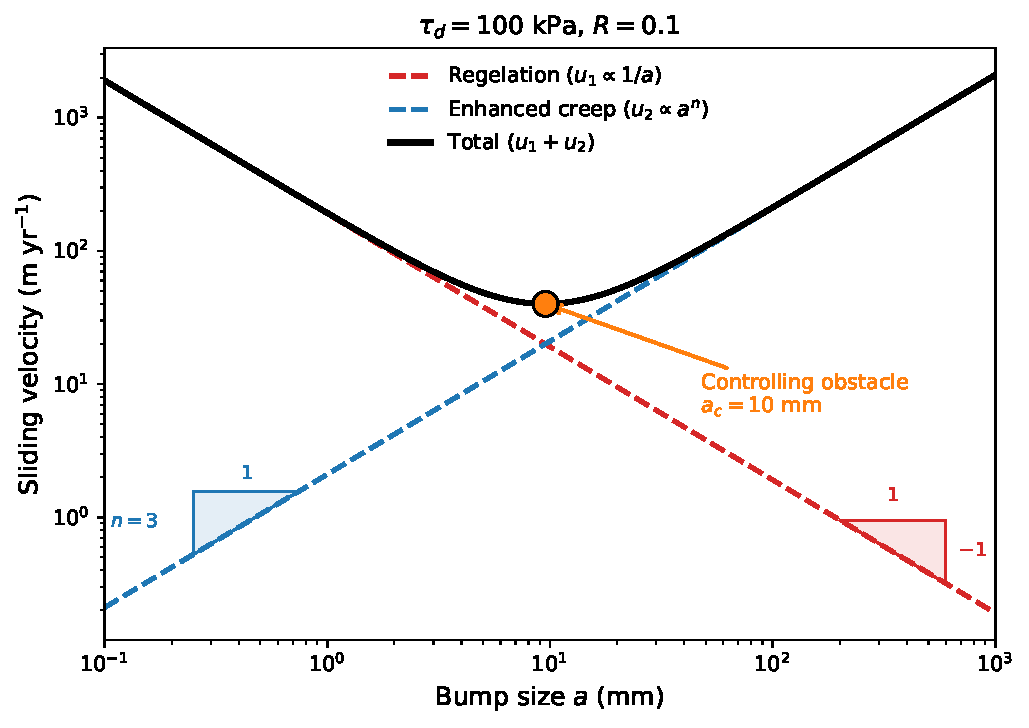
\includegraphics[width=0.75\textwidth]{figures/fig01_regelation_creep_vs_bump_size.pdf}
  \caption{Sliding velocity contributions from regelation ($u_1 \propto 1/a$) and enhanced creep ($u_2 \propto a^n$) as functions of bump size $a$ for $\tau_b = 100$~kPa and roughness $R = 0.1$.  The controlling obstacle size $a_c$ (orange circle) is the bump size at which the total velocity $u_1 + u_2$ is minimized; bumps of this size provide the greatest resistance to sliding.}
  \label{fig:regelation_creep}
\end{figure}

\begin{tcolorbox}[
  colback=blue!5,
  colframe=blue!50!black,
  title={\textbf{Key point: limitations of hard-bed sliding theory}}
]
Weertman-type theories predict sliding velocities that are broadly consistent with observations on slow-sliding mountain glaciers (drag factors $\psi = \tau_b / u_b$ of order 1--20~kPa\,(m\,yr$^{-1}$)$^{-1}$; Table~\ref{tab:drag_factors}).  They fail, however, to explain fast sliding ($u_b > 20$~m\,yr$^{-1}$), because they omit a critical ingredient: water-filled cavities in the lee of bumps.  Fast sliding on a hard bed requires cavities, and cavities require water pressures that approach the ice-overburden pressure.
\end{tcolorbox}

\begin{table}[ht]
\centering
\caption{Apparent drag factors $\psi = \tau_b / u_b$ for selected glaciers, from \cite{CuffeyPaterson2010}.  Glaciers with small $\psi$ (slippery beds) tend to be fast-flowing, marine-terminating, or underlain by deformable sediment.}
\label{tab:drag_factors}
\begin{tabular}{lcccl}
\toprule
\textbf{Glacier} & \textbf{Terminus type} & $\tau_b$ (kPa) & $u_b$ (m\,yr$^{-1}$) & $\psi$ (kPa\,(m\,yr$^{-1}$)$^{-1}$) \\
\midrule
Ice shelves & marine & $\sim$0 & 100--1000 & 0 \\
Whillans Ice Stream & marine & 3 & 400 & 0.008 \\
Columbia Glacier & marine & 100--150 & 1000--2000 & 0.05--0.2 \\
Storglaci\"aren & land & 40 & 30 & 1 \\
Engabreen & land & 100 & 44 & 2 \\
Haut Gl.\ d'Arolla & land & 120 & 6 & 20 \\
\bottomrule
\end{tabular}
\end{table}

%===================================================================
% SECTION 3.3 -- Effective Pressure and Cavities
%===================================================================
\subsection{Effective Pressure and Cavity Formation}
\label{sec:effective_pressure}

The analyses of \S\ref{sec:weertman} assume that all basal water resides in a thin film between ice and rock.  In reality, water also fills cavities in the lee of bedrock bumps.  Cavities reduce the area of contact between ice and bed, effectively reducing the roughness and increasing the sliding velocity.  The formation and evolution of cavities is governed by the \textbf{effective pressure}:
\begin{equation}
  \boxed{N = P_i - P_w = \rho_i\,g\,H - P_w,}
  \label{eq:effective_pressure}
\end{equation}
where $P_i = \rho_i g H$ is the ice-overburden pressure and $P_w$ is the subglacial water pressure.  When $N \to 0$, the glacier approaches flotation and cavities can grow without bound.

\subsubsection{The Separation Pressure}

For a sinusoidal bed with wavelength $\lambda$ and amplitude $a$, the normal stress exerted by the ice on the bed fluctuates about the overburden value $P_i$.  The minimum normal stress---and hence the water pressure at which ice first separates from the bed---is the \textbf{separation pressure}:
\begin{equation}
  P_s = P_i - \frac{\lambda\,\tau_b}{a\,\pi}.
  \label{eq:separation_pressure}
\end{equation}
Cavities begin to form when $P_w$ reaches $P_s$.  The rougher the bed (larger $a/\lambda$), the higher the water pressure required to initiate cavitation.

\subsubsection{Iken's Bound on Basal Drag}

\cite{Iken1981} derived an upper limit on the basal shear stress that a hard bed can support.  For a bed with bumps whose steepest upstream face makes an angle $\beta$ with the mean bed, the critical effective pressure at which sliding becomes unstable is
\begin{equation}
  \boxed{\tau_b = N_c\,\tan\beta,}
  \label{eq:iken_bound}
\end{equation}
where $N_c = P_i - P_c$ is the critical effective pressure.  For a sinusoidal bed, $\tan\beta = 2\pi a / \lambda$, so
\begin{equation}
  P_c = P_i - \frac{\lambda\,\tau_b}{2\pi\,a}.
  \label{eq:critical_pressure}
\end{equation}
This result establishes a fundamental constraint: the drag that a hard bed can exert on the overlying ice is bounded above by a value proportional to the effective pressure and the maximum bed slope.  Once water pressure exceeds $P_c$, a net upward force acts on the ice and sliding becomes unstable---formally analogous to the Coulomb friction criterion for landslides.  \cite{Schoof2005} proved that this bound holds for arbitrary (non-sinusoidal) bed geometries, provided the bed has no vertical faces.

% CHALKBOARD DRAWING 2:
% Sketch Figure 7.4 from C&P: schematic of slip velocity vs. water pressure,
% showing the Weertman regime (P_w < P_s), the cavitation regime (P_s < P_w < P_c),
% and the unstable/globally-controlled limit (P_w -> P_i).

\subsubsection{Sliding with Cavities: Relation Between Drag and Slip}

Combining the physics of enhanced creep, regelation, and cavity formation, the relationship between basal drag $\tau_b$ and slip velocity $u_b$ takes the schematic form shown in Figure~\ref{fig:drag_velocity}:

\begin{enumerate}
  \item At low $u_b$ (no cavities): $\tau_b$ increases with $u_b$ following Weertman-type scaling.
  \item At intermediate $u_b$: cavities form, reducing bed contact and increasing $u_b$ for a given $\tau_b$.  The drag $\tau_b$ reaches a maximum.
  \item At high $u_b$: drag decreases as cavities expand and contact area shrinks, approaching the Iken bound.  The bed can no longer provide sufficient resistance, and the sliding velocity is controlled globally by lateral and longitudinal stresses.
\end{enumerate}

\noindent The existence of a maximum in the $\tau_b$--$u_b$ relation is a robust prediction of all cavity-based sliding theories.  It means that above a certain sliding speed, faster sliding produces \textit{less} drag---a velocity-weakening regime that has important consequences for glacier stability and surge dynamics.

\begin{figure}[ht]
  \centering
  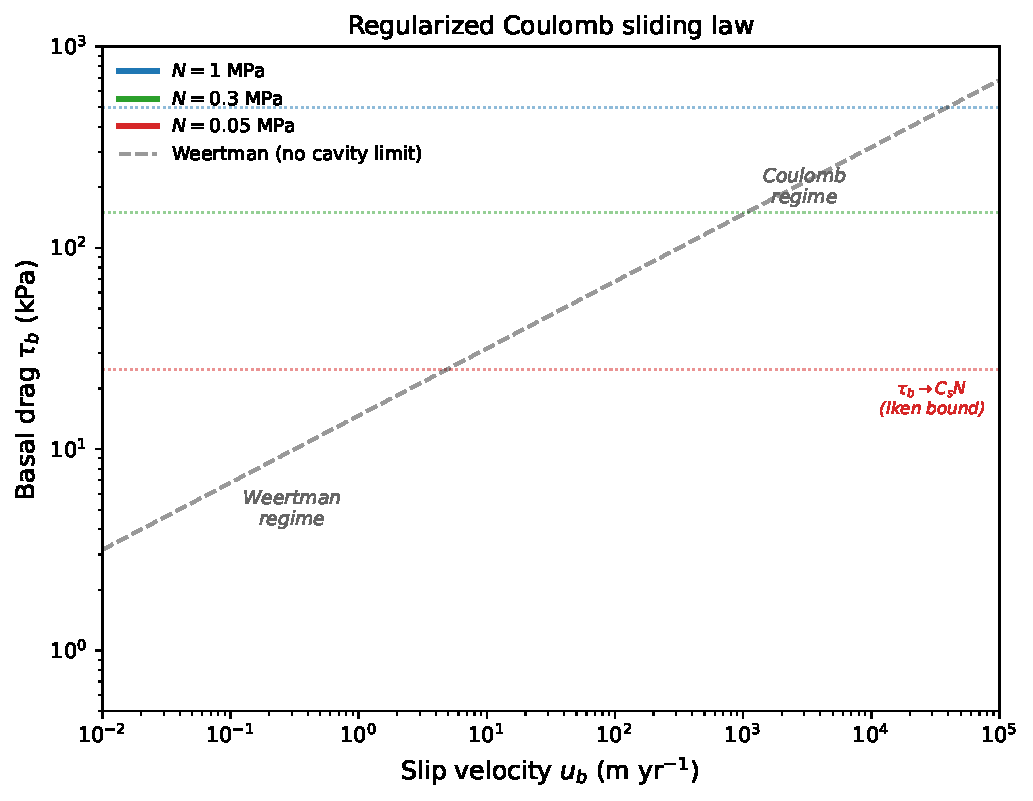
\includegraphics[width=0.75\textwidth]{figures/fig02_drag_vs_slip_velocity.pdf}
  \caption{Basal drag $\tau_b$ vs.\ slip velocity $u_b$ for the regularized Coulomb sliding law at three values of effective pressure $N$.  At low velocities, drag increases following Weertman-type scaling ($\tau_b \propto u_b^{1/n}$).  At high velocities, drag saturates at the Iken/Coulomb bound $\tau_b \to C_s\,N$ (dotted lines), where $C_s = \tan\beta$ is the maximum bed slope.  Lower effective pressure reduces both the drag maximum and the Coulomb limit.}
  \label{fig:drag_velocity}
\end{figure}

\subsection{Observations: Velocity and Water Pressure}
\label{sec:observations_water}

The theoretical expectation that sliding velocity should depend on effective pressure is well supported by observations.  Two classic datasets illustrate this:

\medskip
\noindent\textbf{Findelengletscher} \cite{IkenBindschadler1986}.  Surface velocity and borehole water levels were measured at four lines of stakes over five weeks early in the melt season.  Velocity and water pressure correlate on timescales of days to weeks.  When plotted against effective pressure $N$, velocity varies approximately as $N^{-1}$.

\medskip
\noindent\textbf{Lauteraargletscher} \cite{SugiyamaGudmundsson2004}.  Diurnal cycles of velocity and water pressure show a clear correlation, with a notable asymmetry: sliding is faster when water pressure is rising (and $N$ is decreasing) than when it is falling (and $N$ is increasing) at the same value of $N$.  This hysteresis likely reflects the finite time required for cavities to adjust to changing water pressure---transient cavity growth temporarily contributes to sliding.

\medskip
\noindent\textbf{Bench Glacier} \cite{Harperetal2005,Harperetal2007}.  Two speed-up events were observed in which neither was accompanied by a reduction in effective pressure.  Instead, bed separation increased (indicating cavity growth), but without a decrease in $N$.  This demonstrates that sliding rate can increase without changes in effective pressure, through the redistribution or increased volume of water at the bed.

\begin{tcolorbox}[
  colback=blue!5,
  colframe=blue!50!black,
  title={\textbf{Key point: water pressure is necessary but not sufficient}}
]
Water at the glacier bed increases the sliding rate through at least four mechanisms:
\begin{enumerate}
  \item Low effective pressures allow large cavities, reducing the area of ice--bed contact.
  \item Water can spread across the bed or fill new cavities even without decreasing effective pressure.
  \item Reduced effective pressures decrease frictional drag from rock particles in the basal ice.
  \item Transient cavity growth displaces ice downstream, temporarily increasing the sliding rate.
\end{enumerate}
Both the effective pressure $N$ and the volume of water per unit area of bed must be considered as independent variables in any complete sliding relation.
\end{tcolorbox}

\subsection{Hard-Bed Sliding: Summary}
\label{sec:hard_bed_summary}

The essential features of hard-bed sliding are:

\begin{enumerate}
  \item Ice moves past bedrock bumps by a combination of regelation (dominant for small bumps) and enhanced creep (dominant for large bumps).  The controlling obstacle size---for which both processes are equally effective---is in the range 10--100~mm.

  \item Rapid sliding ($u_b \gtrsim 20$~m\,yr$^{-1}$) on a hard bed requires water-filled cavities in the lee of bumps.  Without cavities, theoretical sliding speeds are much lower than observed.

  \item The drag that a hard bed can support is bounded above by $\tau_b \leq N\,\tan\beta$ (Iken's bound).  As water pressure approaches the overburden, the bed becomes unable to resist the flow and the velocity is controlled by global stresses---lateral drag, longitudinal stresses, and flow over sticky spots elsewhere.

  \item Friction between rock particles in the basal ice and the bedrock can be a significant component of the total drag, potentially equaling or exceeding the drag from regelation and creep around bedrock bumps.  No existing theory provides a complete quantitative treatment of hard-bed sliding that includes regelation, creep, cavitation, rock--rock friction, and water flow simultaneously.
\end{enumerate}

%===================================================================
% SECTION 4 -- Deformable Beds
%===================================================================
\section{Deformable Beds}
\label{sec:soft_bed}

Many glacier beds are not rigid bedrock but consist of unconsolidated sediment---``till'' in glaciological usage.  Deformable beds underlie vast areas of the Pleistocene ice sheets in North America and Europe and are common beneath modern glaciers.  The West Antarctic ice streams, which account for the majority of ice discharge from the West Antarctic Ice Sheet, rest on layers of weak, water-saturated till only a few meters thick.

\subsection{Key Observations}

Table~\ref{tab:deforming_beds} summarizes borehole observations from glaciers known to have deforming beds.  Both soft-bed sliding (at the ice--till interface) and distributed deformation within the till contribute to the total slip rate.  On average, sliding at the interface accounts for the majority of the motion.

\begin{table}[ht]
\centering
\caption{Observations of subglacial deformation from borehole studies.  After \cite{CuffeyPaterson2010}, Table~7.4.}
\label{tab:deforming_beds}
\begin{tabular}{lcccc}
\toprule
\textbf{Glacier} & $u_b$ (m\,yr$^{-1}$) & \textbf{Character} & \textbf{Bed stress} (kPa) & $N$ (kPa) \\
\midrule
Whillans & 400 & $>$80\% sliding & $<$6 & $-20$ to $-150$ \\
Bindschadler & 360 & $<$20\% sliding & $<$10 & 20--40 \\
Columbia & $\sim$2000 & & $\sim$100 & \\
Storglaci\"aren & 15--35 & sliding dominates & 40 & 110 \\
Breidamerkur & $\sim$100 & 10--80\% sliding & 80 & 0--200 \\
\bottomrule
\end{tabular}
\end{table}

\subsection{Till as a Plastic Material}
\label{sec:till_plastic}

Laboratory experiments on subglacial tills consistently show that, after an initial adjustment period, a shearing till attains a yield stress $\tau_*$ that is essentially independent of the deformation rate.  This is the behavior of a \textbf{perfectly plastic material} at a \textbf{critical state}.  The yield stress obeys the Mohr--Coulomb criterion \cite{Iversonetal1998}:
\begin{equation}
  \boxed{\tau_* = c_o + f\,N \approx f\,N,}
  \label{eq:mohr_coulomb}
\end{equation}
where $c_o$ is the apparent cohesion (small for deforming tills), $f = \tan\varphi$ is the friction factor, and $N = \sigma_n - P_w$ is the effective normal stress on the failure plane.  Measured values of $\varphi$ range from about $10^\circ$ to $40^\circ$, giving $f$ in the range 0.17--0.84.  The cohesion is typically small enough to neglect.

\medskip
\noindent The critical implication of equation~\eqref{eq:mohr_coulomb} is that \textbf{the strength of till is controlled by water pressure}.  At effective stresses of order 100~kPa, a till with $\varphi = 30^\circ$ has a yield stress of about 60~kPa.  But if water pressure rises to within a few percent of overburden ($N \to 0$), the till strength drops to near zero and the bed becomes extremely weak.

\begin{table}[ht]
\centering
\caption{Measured strength values for subglacial tills.  After \cite{CuffeyPaterson2010}, Table~7.5.  Values of $\tau_*$ at $N = 50$~kPa are reported where $\varphi$ and $c_o$ were measured.}
\label{tab:till_strength}
\begin{tabular}{lcccl}
\toprule
\textbf{Till} & $\tau_*$ at $N=50$ (kPa) & $\varphi$ & $c_o$ (kPa) & \textbf{Method} \\
\midrule
Whillans Ice Stream & 2--4 & & & lab \\
Storglaci\"aren & 29 & $26^\circ$ & 5 & lab \\
Black Rapids & 43 & $40^\circ$ & 1.3 & lab \\
Breidamerkur & 35 & $32^\circ$ & 3.7 & in situ \\
Two Rivers (Laurentide) & 31 & $18^\circ$ & 14 & lab \\
\bottomrule
\end{tabular}
\end{table}

\begin{figure}[ht]
  \centering
  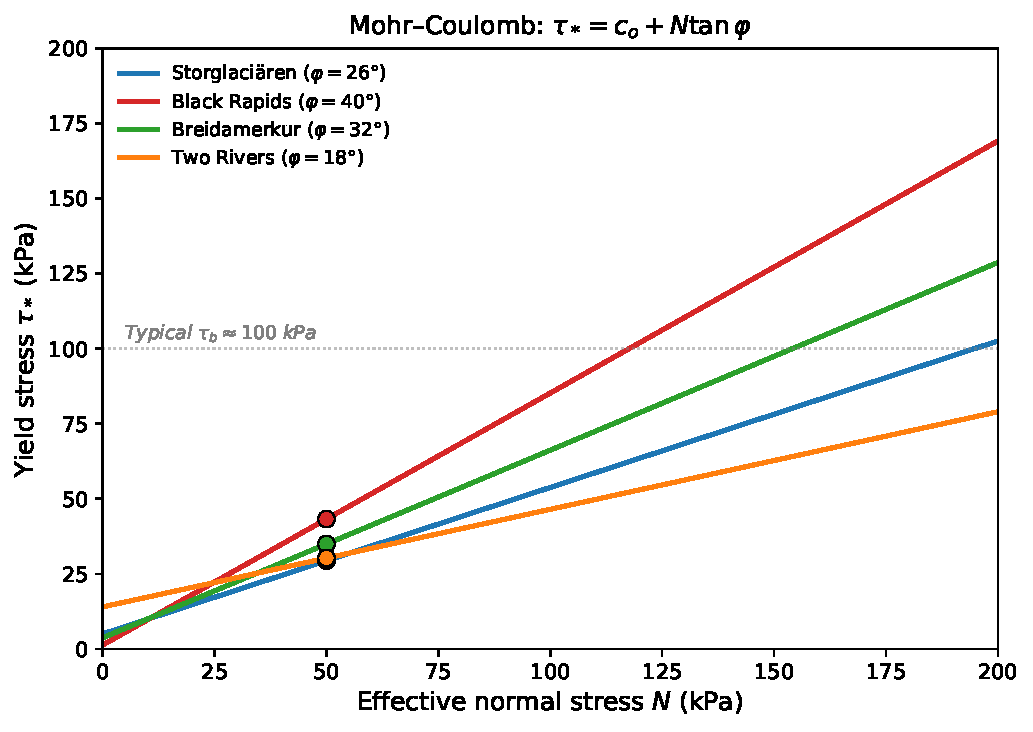
\includegraphics[width=0.75\textwidth]{figures/fig04_mohr_coulomb.pdf}
  \caption{Mohr--Coulomb yield stress $\tau_* = c_o + N\,\tan\varphi$ as a function of effective normal stress $N$ for four subglacial tills with measured friction angles.  Circles mark the yield stress at $N = 50$~kPa.  The horizontal line at $\tau_b = 100$~kPa indicates a typical basal shear stress; tills below this line are too weak to support the applied stress at the corresponding $N$, and the bed will deform.  Data from \cite{CuffeyPaterson2010}, Table~7.5.}
  \label{fig:mohr_coulomb}
\end{figure}

\subsection{Implications of Mohr--Coulomb Behavior}

The Mohr--Coulomb description has several important consequences for glacier dynamics:

\begin{enumerate}
  \item \textbf{Water pressure is the primary control.}  Because $\tau_* \propto N$, the strength of the bed is set almost entirely by the effective pressure.  To produce widespread till deformation beneath a glacier 100~m thick (overburden $\sim$900~kPa), the water pressure must exceed about 83\% of overburden.  Beneath 1~km of ice, the threshold is about 98\% of overburden.  The West Antarctic ice streams, where $P_w$ matches the 9~MPa overburden to within 1\%, are the archetype.

  \item \textbf{Plastic behavior means the drag is bounded.}  A till that behaves plastically cannot support a shear stress greater than $\tau_*$.  If the applied stress exceeds $\tau_*$, the till fails and the glacier accelerates.  This is fundamentally different from a viscous bed, where the drag would increase with velocity.

  \item \textbf{Dilatancy provides a negative feedback.}  When a consolidated till begins to shear, it dilates (expands), creating new pore space.  If water cannot flow in fast enough to fill this new space, the pore pressure drops and $N$ increases, strengthening the till.  This provides a negative feedback that can stabilize deformation.  If, on the other hand, water flows efficiently to the dilating zone, the pressure remains high and deformation continues.

  \item \textbf{Deformation is episodic.}  Subglacial observations show that till deformation varies on timescales of hours to days, is concentrated near the top of the till layer, and often occurs on discrete slip planes rather than as distributed shear.  The rate and location of deformation are sensitive to water pressure fluctuations.
\end{enumerate}

%===================================================================
% SECTION 5 -- Sliding Relations for Models
%===================================================================
\section{Sliding Relations for Glacier Models}
\label{sec:sliding_laws}

Glacier flow models require a relation between basal velocity $u_b$, basal shear stress $\tau_b$, and other variables that serves as the basal boundary condition.  Because no complete theory of basal sliding exists, such relations are necessarily phenomenological.

\subsection{The Weertman Sliding Law}

The simplest and most widely used sliding relation has the form
\begin{equation}
  \boxed{u_b = C\,\tau_b^m,}
  \label{eq:weertman_law}
\end{equation}
where $C$ is a sliding coefficient (inverse of the drag factor) and $m$ is the sliding exponent.  Weertman's theory gives $m = (n+1)/2 \approx 2$ for $n = 3$.  In practice, $m$ and $C$ are treated as tuning parameters.  This law does not include the effect of water pressure and is appropriate only in the local-control regime.

\subsection{Effective-Pressure-Dependent Sliding Laws}

To include the effect of water pressure, the Weertman law is generalized to
\begin{equation}
  u_b = k\,\frac{\tau_b^p}{N^q},
  \label{eq:budd_sliding}
\end{equation}
with $p$ and $q$ positive exponents and $k$ a coefficient that depends on bed properties.  For the simple case $p = 3$ and $q = 1$, this is equivalent to
\begin{equation}
  u_b = k\,\tau_b^3\,N^{-1}.
  \label{eq:budd_n3}
\end{equation}
This form captures the first-order observation that sliding velocity increases with basal shear stress and decreases with effective pressure.  It was used by \cite{Budd1979} and tested against observations of Variegated Glacier following a surge, though no single pair $(p, q)$ could explain velocity variations over both time and space.

\medskip
\noindent In glacier flow models, the Weertman law (equation~\ref{eq:weertman_law}) is often written in its inverse form (basal stress as a function of velocity):
\begin{equation}
  \tau_b = C^{-1/m}\,u_b^{1/m},
  \label{eq:inverse_sliding}
\end{equation}
where the sliding coefficient $C$ absorbs all bed properties including roughness, water pressure, and till strength.  This is the form used in the SSA equations studied in the dynamics lectures.

\subsection{Coulomb-Type Sliding Laws}
\label{sec:coulomb_sliding}

The Mohr--Coulomb behavior of till (\S\ref{sec:till_plastic}) and Iken's bound on hard-bed drag (\S\ref{sec:effective_pressure}) both suggest that the basal shear stress should be bounded by a value proportional to the effective pressure:
\begin{equation}
  \tau_b \leq f\,N.
  \label{eq:coulomb_bound}
\end{equation}
This motivates a Coulomb-type sliding law in which the drag is capped:
\begin{equation}
  \boxed{\frac{\tau_b}{N} = K\,\frac{\tilde{u}^{\,1/n}}{k_0 + \tilde{u}}, \quad \text{where } \tilde{u} = \frac{u_b}{N^{n}},}
  \label{eq:coulomb_sliding}
\end{equation}
following the development in \cite{CuffeyPaterson2010} (equation~7.26).  At low velocities ($\tilde{u} \ll k_0$), $\tau_b \propto u_b^{1/n}$---the Weertman-like regime.  At high velocities ($\tilde{u} \gg k_0$), $\tau_b \to K\,N\,\tilde{u}^{1/n - 1} \to f\,N$---the Coulomb regime, in which drag is controlled by effective pressure and is independent of velocity.

\medskip
\noindent This type of sliding law has two physically desirable features:
\begin{itemize}
  \item It transitions smoothly between velocity-strengthening behavior at low velocities and velocity-independent (plastic) behavior at high velocities.
  \item It ensures that the drag cannot exceed the Iken bound or the Mohr--Coulomb yield stress, providing a physical upper limit on basal resistance.
\end{itemize}

\noindent \cite{Schoof2005} and \cite{Gagliardinietal2007} derived similar relations from first principles for hard beds with cavities, confirming the existence of the drag maximum and the transition to Coulomb-like behavior.

\begin{tcolorbox}[
  colback=orange!25,
  colframe=orange!70!black,
  title={\textbf{Derivation: the Coulomb sliding law from cavity physics}}
]
Consider the simplified model of sliding with cavities from \S\ref{sec:effective_pressure}.  The nominal cavity length is $\ell = n^n\,u_b / (A\,N^n)$, and the shear stress on the remaining contact area is intensified by a factor $(1 + \ell/\lambda_o)$, where $\lambda_o$ is a length scale related to the bed roughness.

\medskip
\noindent Writing $\tilde{u} = u_b / N^n$ and absorbing material constants into $k_0$ and $K$:
\begin{equation}
  \frac{\tau_b}{N} = K\,\frac{\tilde{u}^{1/n}}{k_0 + \tilde{u}}.
\end{equation}
For $n = 3$ and using equation~\eqref{eq:fowler_sliding} for the no-cavity regime, this reproduces the qualitative behavior of Figure~\ref{fig:drag_velocity}: drag increases at low velocity, reaches a maximum at $\tilde{u} = k_0 / (n-1)$, and decreases as $\tilde{u}^{1/n - 1}$ at high velocity (approaching the Iken/Coulomb limit).
\end{tcolorbox}

\begin{figure}[ht]
  \centering
  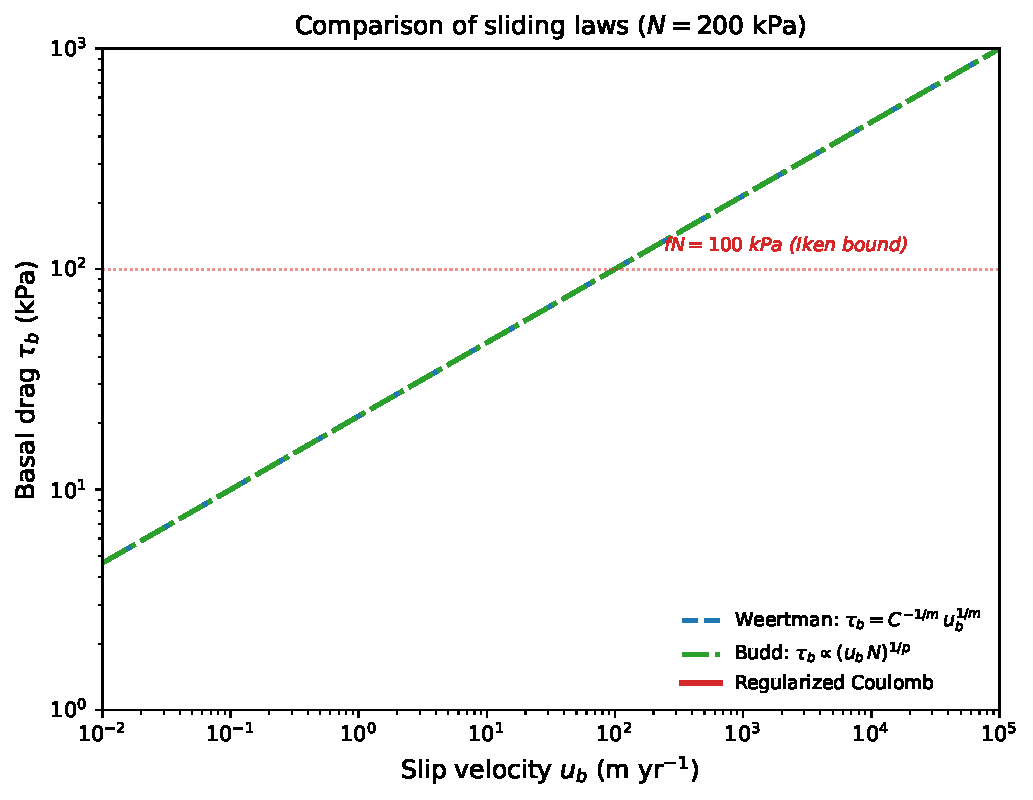
\includegraphics[width=0.75\textwidth]{figures/fig05_sliding_law_comparison.pdf}
  \caption{Comparison of three sliding laws at fixed effective pressure $N = 200$~kPa.  The Weertman law (dashed) and Budd law (dash-dot) both allow drag to grow without bound as velocity increases.  The regularized Coulomb law (solid) transitions from Weertman-like behavior at low velocities to a Coulomb limit $\tau_b \to f\,N$ at high velocities, consistent with Iken's bound and Mohr--Coulomb till behavior.}
  \label{fig:sliding_laws}
\end{figure}

\subsection{Which Law to Use?}

The choice of sliding law depends on the physical setting:

\begin{center}
\begin{tabular}{lll}
\toprule
\textbf{Regime} & \textbf{Appropriate law} & \textbf{Setting} \\
\midrule
Slow sliding, hard bed & Weertman: $u_b = C\,\tau_b^m$ & Mountain glaciers, low $P_w$ \\
Moderate sliding & $u_b = k\,\tau_b^p / N^q$ & Valley glaciers with seasonal $P_w$ \\
Fast sliding, weak bed & $\tau_b = f\,N$ (Coulomb) & Ice streams, near-flotation \\
General & Regularized Coulomb & Transition zones, models \\
\bottomrule
\end{tabular}
\end{center}

\noindent In ice-sheet models, the Weertman law (equation~\ref{eq:weertman_law}) remains the most common choice because of its simplicity and because $C$ can be tuned spatially to match observed velocities.  The Coulomb-type law is increasingly used in studies of marine ice sheets, where effective pressures are low near grounding lines and the Weertman law allows unphysically large drag.

%===================================================================
% SECTION 6 -- Worked Example
%===================================================================
\section{Worked Example: Effective Pressure and Sliding Speed}
\label{sec:example}

Consider a glacier 500~m thick resting on hard bedrock with roughness $R = 0.1$.  The bed has sinusoidal undulations with $\lambda = 10$~m and $a = 1$~m, so $a/\lambda = R$.  The basal shear stress is $\tau_b = 100$~kPa.  We compute the separation pressure, the Iken bound, and the sliding velocity for two values of water pressure.

\medskip
\noindent\textbf{Step 1: Ice-overburden and separation pressures.}
\begin{align}
  P_i &= \rho_i\,g\,H = 917 \times 9.8 \times 500 = 4.49\;\text{MPa}, \\[4pt]
  P_s &= P_i - \frac{\lambda\,\tau_b}{a\,\pi} = 4.49 - \frac{10 \times 0.1}{1 \times \pi} = 4.49 - 0.318 = 4.17\;\text{MPa}.
\end{align}
The water pressure must exceed 4.17~MPa (93\% of overburden) for cavities to form.

\medskip
\noindent\textbf{Step 2: Iken's bound.}  The maximum bed slope is $\tan\beta = 2\pi a/\lambda = 2\pi \times 0.1 = 0.628$, so:
\begin{equation}
  \tau_b^{\max} = N\,\tan\beta = N \times 0.628.
\end{equation}
For the applied $\tau_b = 100$~kPa, sliding becomes unstable when
\begin{equation}
  N < \frac{\tau_b}{\tan\beta} = \frac{100}{0.628} = 159\;\text{kPa}, \quad \text{i.e., } P_w > 4.49 - 0.159 = 4.33\;\text{MPa}.
\end{equation}
At water pressures above 96\% of overburden, the bed can no longer support the applied basal drag.

\medskip
\noindent\textbf{Step 3: Sliding velocities.}  Using the effective-pressure-dependent law $u_b = k\,\tau_b^3\,N^{-1}$ with $k = 3.5 \times 10^{-16}$~m\,Pa$^{-2}$\,s$^{-1}$ (a representative value):

\begin{center}
\begin{tabular}{cccc}
\toprule
$P_w$ (MPa) & $P_w / P_i$ & $N$ (MPa) & $u_b$ (m\,yr$^{-1}$) \\
\midrule
3.59 & 80\% & 0.90 & 12 \\
4.26 & 95\% & 0.22 & 50 \\
4.40 & 98\% & 0.09 & 123 \\
\bottomrule
\end{tabular}
\end{center}

\begin{figure}[ht]
  \centering
  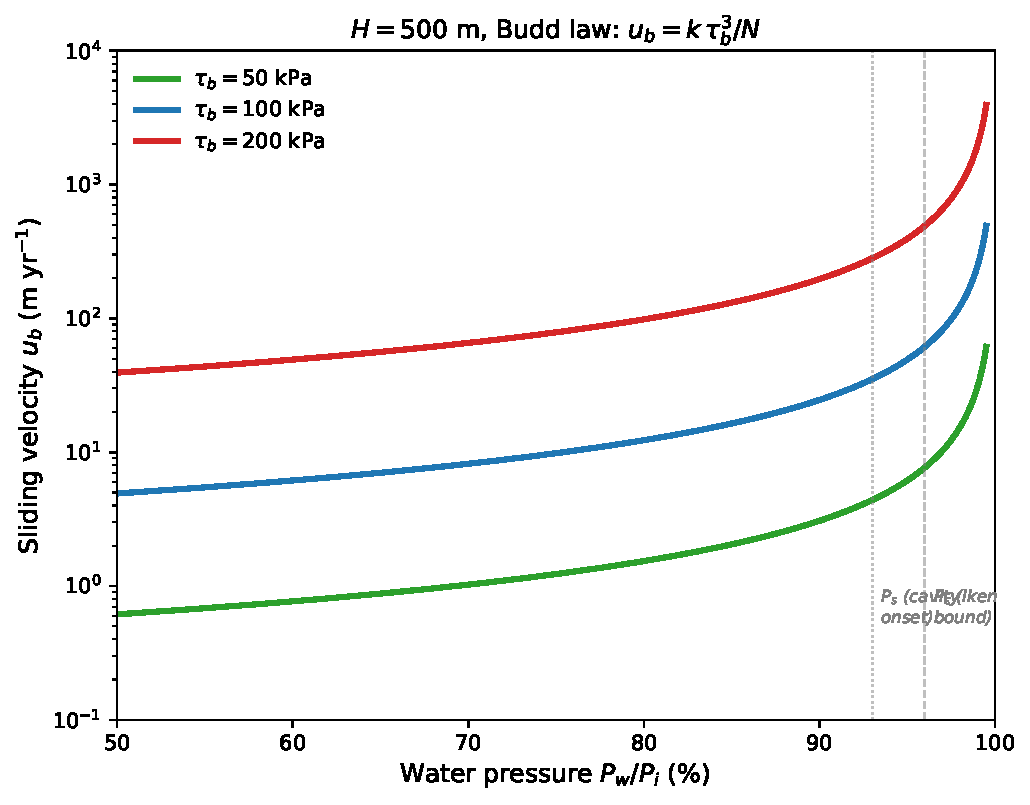
\includegraphics[width=0.75\textwidth]{figures/fig03_velocity_vs_effective_pressure.pdf}
  \caption{Sliding velocity as a function of water pressure (expressed as a fraction of ice-overburden pressure) for the Budd-type sliding law $u_b = k\,\tau_b^3 / N$ at three values of basal shear stress.  The vertical dotted lines mark the approximate separation pressure $P_s$ (onset of cavitation) and the critical pressure $P_c$ (Iken bound) for the bed geometry of the worked example.  Sliding speed increases by more than an order of magnitude as water pressure rises from 80\% to 98\% of overburden.}
  \label{fig:velocity_vs_N}
\end{figure}

\noindent Increasing the water pressure from 80\% to 98\% of overburden increases the sliding speed by an order of magnitude.  This extreme sensitivity to water pressure is why the subglacial hydrological system---which controls the distribution and magnitude of $P_w$---is a first-order control on glacier dynamics.

\clearpage
%===================================================================
% Reading
%===================================================================
\section*{Reading}

Cuffey \& Paterson, \textit{Physics of Glaciers}, 4th ed.:
\begin{itemize}
  \item Section 7.1: Introduction and measurements of basal velocity
  \item Section 7.2: Hard beds---Weertman's theory, cavities, water pressure, and Iken's bound
  \item Section 7.3: Deformable beds---till properties and Mohr--Coulomb behavior
\end{itemize}

%===================================================================
% Bibliography
%===================================================================
\bibliographystyle{plainnat}
\bibliography{../references}

\end{document}
